\originalchapter{习题课五: 安培定律}
题源为\href{https://ocw.mit.edu/courses/8-02-physics-ii-electricity-and-magnetism-spring-2007/resources/solving05/}{Problem Solving 5}, PDF第1--10页(原页脚误沿用Solving 6). 全部Q1--Q18和同轴电缆考试练习题保留. 所有解答为AI独立解答.

\begin{exercise}
情境一. 无限长圆柱导体有空心轴, 内半径$a$、外半径$b$, 总电流$I$沿正$z$, 在铜截面中均匀分布. 对$a<r<b$取半径$r$安培圆.
Q1求电流密度及包围电流.
Q2用包围面积占比再求包围电流.
Q3核$r=a,b$时的包围电流并解释.
Q4写磁场环量.
Q5求壁内场.
Q6求$r<a$场.
Q7求$r>b$场.
Q8画场大小图. 同时说明对称性、方向和三个区域.
\end{exercise}
\begin{solution}
Q1--2. $J=I/[\pi(b^2-a^2)]$, $I_{\rm enc}=J\pi(r^2-a^2)=I(r^2-a^2)/(b^2-a^2)$. 后一因子也正是被包围铜面积占总铜面积的比例.
Q3. $r=a$未包围铜截面, 电流为零; $r=b$包围全部截面, 为$I$.
Q4. 圆对称使$\bb=B\uv\phi$, 从正$z$看为逆时针, 环量$2\pi rB$.
Q5--7. 由安培定律得到
\[
B(r)=\begin{cases}0,&r<a,\\
\displaystyle\frac{\mu_0I(r^2-a^2)}{2\pi r(b^2-a^2)},&a<r<b,\\
\displaystyle\frac{\mu_0I}{2\pi r},&r>b.
\end{cases}
\]
Q8. 空心区为零, 壁内从零单调增至$\mu_0I/(2\pi b)$, 然后按$1/r$下降, 两个边界连续.
\begin{center}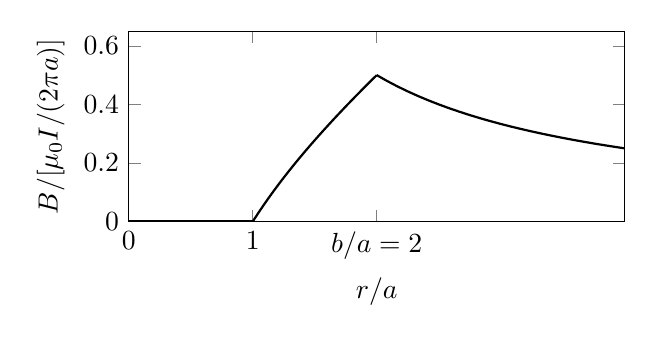
\begin{tikzpicture}
\begin{axis}[width=.65\linewidth,height=4cm,xlabel={$r/a$},ylabel={$B/[\mu_0I/(2\pi a)]$},xmin=0,xmax=4,ymin=0,ymax=.65,xtick={0,1,2},xticklabels={0,1,$b/a=2$}]
\addplot[thick,domain=0:1]{0};\addplot[thick,domain=1:2]{(x^2-1)/(3*x)};\addplot[thick,domain=2:4]{1/x};
\end{axis}\end{tikzpicture}\end{center}
此图选$b/a=2$作无量纲示意.
\end{solution}

\begin{exercise}
情境二. 厚度$d$、沿$x,z$无限延展的电流板占$|y|<d/2$, 在$x,z$方向无限, 电流密度为$\jj=(2J_e|y|/d)\uv z$, $J_e$单位A/m$^2$.
Q9求中心场.
Q10为$y>d/2$选并画安培回路, 标尺寸.
Q11求包围电流.
Q12求环量.
Q13求板外场.
Q14为$0<y<d/2$选并画回路.
Q15求包围电流.
Q16求环量.
Q17求板内场.
Q18依对称性求$y<0$场, 画有符号$B_x(y)$图并标轴. 另说明方向及矩形对称.
\end{exercise}
\begin{solution}
Q9. $J(y)$偶对称, 上下薄电流面在中心相消, $\bb(0)=0$.
Q10--12. 在$xy$平面取宽$h$、高$y$矩形, 底边$y=0$, 顶边在所求$y>d/2$. 环路正法向取$+z$, 故顶边沿$-x$. 包围电流$h\int_0^{d/2}(2J_ey'/d)\dd y'=hJ_ed/4$. 竖边与场垂直, 底边场零, 环量为$-hB_x(y)$.
Q13. $B_x(y)=-\mu_0J_ed/4$.
Q14--16. 同样矩形但顶边在板内$y$, 包围电流$hJ_ey^2/d$, 环量仍为$-hB_x$.
Q17--18. 因而
\[
B_x(y)=\begin{cases}\displaystyle-\frac{\mu_0J_e}{d}y|y|,&|y|<d/2,\\
\displaystyle-\frac{\mu_0J_ed}4\operatorname{sgn}(y),&|y|>d/2.
\end{cases}
\]
上半部向$-x$, 下半部向$+x$. 原题密度有绝对值, 因而两半的电流均沿$+z$, 不可替换成一半反向电流.
\begin{center}\begin{tikzpicture}[>=Stealth]
\draw[->](-.3,0)--(3.3,0) node[right]{$x$};\draw[->](0,-.4)--(0,2.1)node[above]{$y$};
\draw[thick,->](.4,0)--(2.6,0);\draw[thick,->](2.6,0)--(2.6,1.5);\draw[thick,->](2.6,1.5)--(.4,1.5);\draw[thick,->](.4,1.5)--(.4,0);
\node at(1.5,-.35){$h$};\node[right]at(2.6,.8){$y$};\node at(1.5,.7){法向$+z$};
\end{tikzpicture}\quad
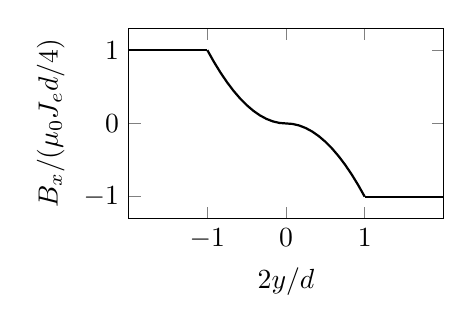
\begin{tikzpicture}\begin{axis}[width=.46\linewidth,height=4cm,xlabel={$2y/d$},ylabel={$B_x/(\mu_0J_ed/4)$},xmin=-2,xmax=2,ymin=-1.3,ymax=1.3,xtick={-1,0,1},ytick={-1,0,1}]
\addplot[thick,domain=-2:-1]{1};\addplot[thick,domain=-1:1]{-x*abs(x)};\addplot[thick,domain=1:2]{-1};
\end{axis}\end{tikzpicture}\end{center}
\end{solution}

\begin{exercise}
考试练习题. 同轴电缆内实心导体半径$a$, 外导体内外半径$b,c$, 两导体均匀分布相反电流$\pm I_0$, 内导体沿$+z$. (a)求$r<a$场; (b)求$a<r<b$场; (c)求$b<r<c$场; (d)画磁场大小并标轴, 在各区画安培圆. 同时补写外部$r>c$场.
\end{exercise}
\begin{solution}
各区均选半径$r$同轴圆, 环量$2\pi rB$. 图中实线为导体截面边界, 三个虚线圈分别在(a)、(b)、(c)区, 均从正$z$方向看.
\begin{center}\begin{tikzpicture}[scale=.65,>=Stealth]
\foreach \rad in {1,2,3}{\draw[thick](0,0)circle(\rad);}
\foreach \rad/\ang/\lab in {.6/45/{(a)},1.5/135/{(b)},2.5/225/{(c)}}{\draw[dashed,structurecolor](0,0)circle(\rad);\node at(\ang:\rad+.2){\lab};\draw[->,structurecolor](0:\rad)arc(0:25:\rad);}
\node[right]at(1,0){$a$};\node[right]at(2,0){$b$};\node[right]at(3,0){$c$};
\end{tikzpicture}\end{center}
包围电流分别为$I_0r^2/a^2,I_0,I_0[1-(r^2-b^2)/(c^2-b^2)],0$. 所以
\[
B(r)=\frac{\mu_0I_0}{2\pi}\begin{cases}r/a^2,&r<a,\\1/r,&a<r<b,\\(c^2-r^2)/[r(c^2-b^2)],&b<r<c,\\0,&r>c.\end{cases}
\]
场均沿$\uv\phi$或为零. 三个边界连续; 外导体内部抵消包围电流而逐渐降至零.
\begin{center}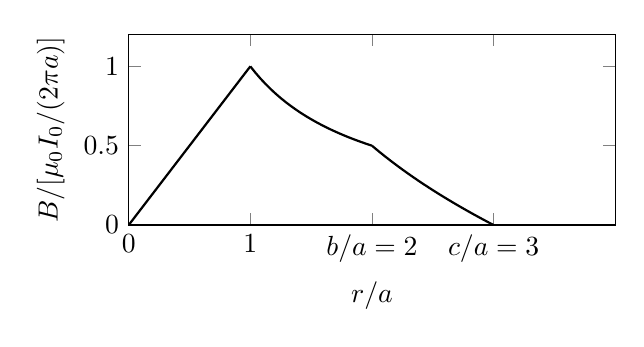
\begin{tikzpicture}\begin{axis}[width=.64\linewidth,height=4cm,xlabel={$r/a$},ylabel={$B/[\mu_0I_0/(2\pi a)]$},xmin=0,xmax=4,ymin=0,ymax=1.2,xtick={0,1,2,3},xticklabels={0,1,$b/a=2$,$c/a=3$}]
\addplot[thick,domain=0:1]{x};\addplot[thick,domain=1:2]{1/x};\addplot[thick,domain=2:3]{(9-x^2)/(5*x)};\addplot[thick,domain=3:4]{0};
\end{axis}\end{tikzpicture}\end{center}
图中半径比仅为示意取值.
\end{solution}
